\documentclass[mathserif, handout]{beamer}
% ======================================================================
% General LaTeX Setup for Beamer (Reusable Preamble)
% Author: Chandra Gummaluru
% ======================================================================

\documentclass[mathserif, handout]{beamer}
\setbeamertemplate{frametitle}{}

% ------------------------------------------------------------
% basic packages
% ------------------------------------------------------------
\usepackage{url}
\usepackage{ifthen}
\usepackage{enumerate}
\usepackage[font=small]{caption}
\usepackage{subcaption}
\usepackage{moresize}
\usepackage[outline]{contour}
\usepackage{transparent}
\usepackage{worldflags}
\usepackage{bm}
\usepackage{graphbox}
\usepackage{mathtools}
\usepackage{multirow}
\usepackage{fontawesome5}
\usepackage{pifont}
\usepackage{array}
\usepackage{comment}

% ------------------------------------------------------------
% math
% ------------------------------------------------------------
\DeclarePairedDelimiter{\floor}{\lfloor}{\rfloor}
\DeclarePairedDelimiter{\ceil}{\lceil}{\rceil}

% ------------------------------------------------------------
% colors
% ------------------------------------------------------------
\definecolor{hl}{RGB}{248,196,69}
\definecolor{myred}{HTML}{ED5565}
\definecolor{myorange}{HTML}{FC6E51}
\definecolor{myyellow}{HTML}{FFCE54}
\definecolor{mycyan}{HTML}{4FC1E9}
\definecolor{myblue}{HTML}{5D9CEC}

\newcommand{\graytext}[1]{\footnotesize\color{gray}#1\normalsize\color{black}}

% ------------------------------------------------------------
% symbols
% ------------------------------------------------------------
\newcommand{\cmark}{\ding{51}}
\newcommand{\xmark}{\ding{55}}

% ------------------------------------------------------------
% highlighting
% ------------------------------------------------------------
\newcommand{\reducedstrut}{\vrule width 0pt height .9\ht\strutbox depth .9\dp\strutbox\relax}
\newcommand{\highlight}[1]{%
  \begingroup\setlength{\fboxsep}{0pt}\colorbox{hl}{\reducedstrut$\displaystyle #1$\/}\endgroup}
\newcommand{\highlightc}[2]{%
  \begingroup\setlength{\fboxsep}{0pt}\colorbox{#1}{\reducedstrut$\displaystyle #2$\/}\endgroup}

% ------------------------------------------------------------
% environments (boxes)
% ------------------------------------------------------------
\usepackage{tcolorbox}
\tcbuselibrary{skins}

\newtcolorbox{thmbox}[1][]{colback=gray!30!white!20, colframe=black, fonttitle=\bfseries, title=#1, boxrule=0.5pt}

% 1) Bottom open (draw top + sides only)
\newtcolorbox{thmboxtop}[1][]{
    enhanced,
    frame hidden,
    colback=gray!30!white!20,
    borderline north={0.5pt}{0pt}{black}, % top
    borderline west={0.5pt}{0pt}{black},  % left
    borderline east={0.5pt}{0pt}{black}   % right
}

% 2) Top open (draw bottom + sides only)
\newtcolorbox{thmboxbot}[1][]{
    enhanced,
    frame hidden,
    colback=gray!30!white!20,
    borderline south={0.5pt}{0pt}{black}, % bottom
    borderline west={0.5pt}{0pt}{black},  % left
    borderline east={0.5pt}{0pt}{black}   % right
}

% 3) Side only (draw only left and right)
\newtcolorbox{thmboxside}[1][]{
    enhanced,
    frame hidden,
    colback=gray!30!white!20,
    borderline west={0.5pt}{0pt}{black},  % left
    borderline east={0.5pt}{0pt}{black}   % right
}

\newtcolorbox{defboxtop}[1][]{
    enhanced,
    colback=gray!30!white!20,
    frame hidden,
    overlay={
        % Draw top + sides with rounded corners
        \draw[line width=0.5pt, black, rounded corners=3mm]
            (frame.south west) -- (frame.north west) -- (frame.north east) -- (frame.south east);
    },
    #1
}

\newtcolorbox{defboxbot}[1][]{
    enhanced,
    colback=gray!30!white!20,
    frame hidden,
    overlay={
        % Draw top + sides with rounded corners
        \draw[line width=0.5pt, black, rounded corners=3mm]
            (frame.north west) -- (frame.south west) -- (frame.south east) -- (frame.north east);
    },
    #1
}

\newtcolorbox{defboxside}[1][]{
    enhanced,
    frame hidden,
    colback=gray!30!white!20,
    borderline west={0.5pt}{0pt}{black},  % left
    borderline east={0.5pt}{0pt}{black}   % right
}

\newtcolorbox{proofbox}[1][]{colback=gray!20!white!20, colframe=grey, fonttitle=\bfseries, title=#1, boxrule=0.5pt, colbacktitle=white, enhanced jigsaw, sharp corners}

% ------------------------------------------------------------
% code listings
% ------------------------------------------------------------
\usepackage{listings}
\lstdefinestyle{mypython}{
  language=Python,
  deletekeywords=[2]{open, next, from, chr, str, int},
  morekeywords=[3]{List, Graph, Tree, Dict, Set, UnionFind, Ordict, Trie, Queue},
  morekeywords=[4]{ListNode, Vertex, Edge, Path, TreeNode, DictNode, UnifNode, OrdictNode, TrieNode, QueueNode},
  morekeywords=[5]{True, False, Boolean, String, Integer, Key, Function, KeyedObject, Object, Array, Tuple, Optional, None},
  keywordstyle=\color{mycyan}\bfseries,
  keywordstyle=[3]\color{myblue}\bfseries,
keywordstyle=[4]\color{myblue}\bfseries,
keywordstyle=[5]\color{mycyan}\bfseries,
  stringstyle=\color{orange},
  commentstyle=\color{gray}\itshape,
  basicstyle=\ttfamily\footnotesize,
  numbers=left,
  numberstyle=\tiny\color{gray},
  stepnumber=1,
  numbersep=5pt,
  xleftmargin=15pt,
  frame=none,
  showstringspaces=false,
  breaklines=true,
  breakatwhitespace=true,
  tabsize=4,
  columns=flexible
}


% ------------------------------------------------------------
% algorithms
% ------------------------------------------------------------
\usepackage{algorithm}
\usepackage[endLComment=~]{algpseudocodex}
\makeatletter
\algrenewcommand\ALG@beginalgorithmic{\footnotesize}
\makeatother

% ------------------------------------------------------------
% optimization environments
% ------------------------------------------------------------
\usepackage[nocomma]{optidef}

% ------------------------------------------------------------
% pgfplots and pie charts
% ------------------------------------------------------------
\usepackage{pgfplots}
\usepackage{pgf-pie}
\pgfplotsset{compat=1.7}

% ------------------------------------------------------------
% tikz
% ------------------------------------------------------------
\usepackage{tikz}
\usetikzlibrary{
  angles, quotes, positioning, fit, backgrounds, shapes.geometric, intersections,
  calc, shapes, mindmap, decorations.text, arrows, arrows.meta,
  automata, chains, decorations.pathreplacing, calligraphy,
  decorations.markings, shapes.misc, decorations.pathmorphing
}
\tikzset{
  invisible/.style={opacity=0},
  visible on/.style={alt=#1{}{invisible}},
  alt/.code args={<#1>#2#3}{\alt<#1>{\pgfprioritysalso{#2}}{\pgfprioritysalso{#3}}}
}

\newcommand{\multiedge}[5][]{
\pgfmathsetmacro{\N}{#4}
\pgfmathsetmacro{\mid}{(\N-1)/2}
\foreach \i in {0,...,\numexpr#4-1\relax} {

\pgfmathsetmacro{\k}{\i-\mid}
\draw[#1] ($ (#2) + \k*#5*($(#2)!1!90:(#3)$) $) -- ($ (#3) + \k*#5*($(#2)!1!90:(#3)$) $); 

}
\draw[#1,  -{>[scale=1]}]
  ($(#2)!0.54!(#3)$) -- ($(#2)!0.55!(#3)$);
}

% ------------------------------------------------------------
% bibliography
% ------------------------------------------------------------
\usepackage[style=ieee]{biblatex}
\setbeamertemplate{bibliography item}{\insertbiblabel}
\setbeamertemplate{background canvas}{
  \begin{tikzpicture}[remember picture,overlay]
    \node[opacity=0.0075]
      at (current page.center)
      {
\includegraphics[width=0.8\paperwidth]{images/signature.pdf}};
  \end{tikzpicture}
}

% ------------------------------------------------------------
% beamer theme and settings
% ------------------------------------------------------------
\usetheme{Boadilla}
\usecolortheme{seagull}
\beamertemplatenavigationsymbolsempty
\setbeamertemplate{enumerate item}{(\arabic{enumi})}
\setbeamertemplate{enumerate subitem}{(\alph{enumii})}
\setbeamertemplate{enumerate subsubitem}{(\roman{enumiii})}
\setbeamertemplate{itemize item}[circle]
\setbeamertemplate{itemize subitem}{\circ}
\setbeamertemplate{itemize subsubitem}{-}
\setbeamercolor{item}{fg=black!40}
\setbeamercovered{transparent=10}

% ===========================
% Premade TikZ Figure Commands
% ===========================

% images w/ labels
% inside tikz as a node
\NewDocumentCommand{\labeledimgnodetikz}{O{} m m m m m m}{%
	\begin{scope}[transparency group, #1]
		\node[
			draw,
			circle,
			inner sep=0,
			outer sep=0,
			minimum size=10mm,
			#1
		] (#5) at (#3,#4)
		{\includegraphics[scale=#7]{#6}};
		\node[
			rectangle,
			draw=black,
			thick,
			fill=black!55,
			rounded corners=0.1mm,
			inner sep=0pt,
			outer sep=0pt,
			minimum size=2.8mm,
			minimum width=3.5mm
		] at (#3,#4-0.1) {};
		\node[outer sep=0, inner sep=0, white] at (#3,#4-0.1) {\footnotesize #2};
	\end{scope}
}

% inside tikz isolated

% outside tikz
\NewDocumentCommand{\labelednode}{m}{%
	\begin{tikzpicture}[baseline={(0,-1mm)}]
		\node[
			rectangle,
			thick,
			draw=black,
			fill=black!55,
			rounded corners=0.1mm,
			inner sep=0pt,
			outer sep=0pt,
			minimum size=2.8mm,
			minimum width=3.5mm
		] at (0,0) {};
		\node[outer sep=0, inner sep=0, white, minimum size=2.8mm, minimum width=3.5mm] at (0,0) {\footnotesize #1};
	\end{tikzpicture}
}

% images only
% inside tikz as a node
\NewDocumentCommand{\imgnodetikz}{O{} m m m m m m}{%
	\begin{scope}[transparency group, #1]
		\node[
			draw,
			circle,
			inner sep=0,
			outer sep=0,
			minimum size=10mm,
			#1
		] (#5) at (#3,#4)
		{\includegraphics[scale=#7]{#6}};
		\node[
			rectangle,
			draw,
			thick,
			fill=black!55,
			rounded corners=0.1mm,
			inner sep=0pt,
			outer sep=0pt,
			minimum size=2.8mm,
			minimum width=3.5mm,
			opacity=0
		] at (0,0) {};
		\node[outer sep=0, inner sep=0, white, opacity=0] at (0,0) {\footnotesize #2};
	\end{scope}
}

% inside tikz isolated
\NewDocumentCommand{\imgtikz}{O{} mm}{%
	\begin{scope}[transparency group, #1]
		\node[
			inner sep=0,
			outer sep=0
		] (#5) at (#3,#4)
		{\includegraphics[scale=#3]{#2}};
	\end{scope}
}


% outside tikz
\NewDocumentCommand{\imgnode}{mm}{%
	\begin{tikzpicture}[baseline={(0,-1mm)}]
        \node[
            inner sep=0,
            outer sep=0,
            draw opacity=0,
        ] at (0,0)
        {\includegraphics[scale=#2]{#1}};
    \end{tikzpicture}
}

% outside tikz (inline)
\newcommand{\imgnodetext}[2]{%
	\hspace{-0.5mm}%
	\raisebox{-0.26\height}{%
		\includegraphics[scale=#2]{#1}%
	}%
	\hspace{-0.5mm}%
}


% labels only
% inside tikz as a node
\NewDocumentCommand{\labeltikz}{m}{%
	\node[
		rectangle,
		thick,
		draw=black,
		fill=black!55,
		rounded corners=0.1mm,
		inner sep=0pt,
		outer sep=0pt,
		minimum size=2.8mm,
		minimum width=3.5mm
	] at (0,0) {};
	\node[outer sep=0, inner sep=0, white, draw opacity=0] at (0,0) {\footnotesize #1};
}

% inside tikz isolated

% outside tikz

% === define custom pgfkeys ===
\pgfkeys{
	/devicenode/.is family, /devicenode,
	outline thickness/.initial=thick,
	outline color/.initial=black
}

\NewDocumentCommand{\qpacket}{m}{%
	\begin{tikzpicture}[baseline=(current bounding box.center)]
		\node at (0.5,0.4) {\includegraphics[scale=0.1]{#1}};
	\end{tikzpicture}%
}

\NewDocumentCommand{\bpacketid}{mmm}{%
	\begin{tikzpicture}[baseline=(current bounding box.center)]
		\begin{scope}[shift={(0.85,0.7)}]
			\draw[thick, draw=black, fill=#1, rounded corners=1pt] (0.01,0.05) rectangle node[white, text width=1cm, align=center] {\color{#3}\footnotesize #2} (-0.71,-0.625);
		\end{scope}
	\end{tikzpicture}%
}

\NewDocumentCommand{\packetid}{mmmm}{%
	\begin{tikzpicture}[baseline=(current bounding box.center)]
		\begin{scope}[shift={(0.85,0.7)}]
			\draw[thick, draw=black, fill=#2, rounded corners=1pt] (0.01,0.05) rectangle node[white, text width=1cm, align=center] {\color{#4}\footnotesize #3} (-0.71,-0.625);
			\node[
				star,
				star points=30,
				star point ratio=0,
				scale=1.5,
				draw=black,
				thick,
				fill=white,
				rounded corners=0.1mm,
				inner sep=0pt,
				minimum size=2.8mm
			] at (0,0) {};
			\node at (0,0) {\footnotesize #1};
		\end{scope}
	\end{tikzpicture}%
}

\tikzset{
	dictnode/.pic={
			\draw[thick, fill=#1, line join=]
			(-0.75,-0.5) --
			(-0.75,0.5)  --
			(0.75,0.5) --
			(0.75,-0.5) --
			cycle --
			(-0.75, 0.75) --
			(0.75, 0.75) --
			(0.75, -0.5) --
			cycle;
		}
}

\tikzset{
	queuenode/.pic={
			\draw[thick, fill=#1, line join=round]
			(-0.85,-0.5) --
			(-0.85,0.5)  --
			(0.65,0.5) --
			(0.75,0) --
			(0.65,-0.5) --
			cycle;
		}
}

\tikzset{
	queuenodetail/.pic={
			\draw[thick, fill=#1, line join=round]
			(-0.75,-0.5) --
			(-0.75,0.5)  --
			(0.65,0.5) --
			(0.75,0) --
			(0.65,-0.5) --
			cycle;
		}
}

\tikzset{
	listnode/.style={
			shape=rectangle,
			rounded corners,
			thick,
			minimum height=10mm,
			minimum width=15mm,
			inner sep=0pt
		}
}

\tikzset{
	arraynode/.style={
			shape=rectangle,
			thick,
			minimum height=10mm,
			minimum width=15mm,
			inner sep=0pt
		}
}

\tikzset{
	graphnode/.style={
			shape=circle,
			thick,
			minimum size=5mm,
			inner sep=0pt
		}
}

\tikzset{
	defaultnode/.style={
			transform shape,
			circle,
			draw=black,
			thick,
			fill=white,
			minimum size=10mm,
			inner sep=0pt
		},
	newnode/.style={
			transform shape,
			defaultnode,
			draw=myyellow,
			fill=myyellow!60,
			very thick
		},
	newnodelight/.style={
			transform shape,
			defaultnode,
			draw=myyellow,
			fill=myyellow!30,
			very thick
		},
	deletenode/.style={
			defaultnode,
			draw=gray,
			dashed,
			fill=lightgray,
			text=gray,
			very thick
		},
	nooutlinenode/.style={
			defaultnode,
			draw=none,
            draw opacity=0,
			text=black,
			very thick
		},
    nofillnode/.style={
			defaultnode,
			fill=none,
            text=black,
			very thick
		}
}
\tikzset{
	faded/.style={opacity=0.5, text opacity=0.5, transparency group}
}
\tikzset{
	smallgraytext/.style={font=\footnotesize\color{gray}}
}
\tikzset{
	graytext/.style={font=\normalsize\color{gray}}
}
\tikzset{
  squigglearrow/.style={
    very thick,
    lightgray,
    decorate,
    decoration={
      snake,
      amplitude=1.75pt,
      segment length=8pt
    }
  }
}



% title
\title{Trees}
\subtitle{Algorithms and Data Structures}
\author[C. Gummaluru]{Chandra Gummaluru}
\titlegraphic{
\includegraphics[width=0.15\linewidth]{images/signature.pdf}}
\institute[]{\url{chandra-gummaluru.github.io} }
\date[Algorithms and Data Structures]{}

\begin{document}

% beamer
\beamertemplatenavigationsymbolsempty
\setbeamertemplate{enumerate item}{(\arabic{enumi})}
\setbeamertemplate{enumerate subitem}{(\alph{enumii})}
\setbeamertemplate{enumerate subsubitem}{(\roman{enumiii})}

\setbeamertemplate{itemize item}[circle]
\setbeamertemplate{itemize subitem}{\circ}
\setbeamertemplate{itemize subsubitem}{-}
\setbeamercolor{item}{fg=black!40}

\setbeamercovered{transparent=10}

% pgfplots
\pgfplotsset{compat=1.7}

% tikz
\tikzset{
  invisible/.style={opacity=0},
  visible on/.style={alt=#1{}{invisible}},
  alt/.code args={<#1>#2#3}{%
      \alt<#1>{\pgfkeysalso{#2}}{\pgfkeysalso{#3}}
    },
}

\begin{frame}
  \maketitle
\end{frame}

\begin{frame}{Motivation}
  \begin{center}
    \Large \highlight{\textbf{motivation}}
  \end{center}
\end{frame}

\begin{frame}
  A device (\imgnodetext{images/server.png}{0.0325}) wants to send (or broadcast) the same message to all other devices on the same network.
  \begin{figure}
    \centering
    \begin{tikzpicture}[scale=0.8, transform shape]
      \draw[opacity=0] (-2, -2.5) rectangle (11.25,4.75);
      \labeledimgnodetikz[defaultnode]{\footnotesize\texttt{A}}{1.5}{2}{tA}{images/radio_tower.png}{0.044};
      \labeledimgnodetikz[defaultnode]{\footnotesize\texttt{B}}{3}{0}{tB}{images/radio_tower.png}{0.044};
      \labeledimgnodetikz[defaultnode]{\footnotesize\texttt{C}}{4}{2}{tC}{images/radio_tower.png}{0.044};
      \labeledimgnodetikz[defaultnode]{\footnotesize\texttt{D}}{6}{0.5}{tD}{images/radio_tower.png}{0.044};
      \labeledimgnodetikz[defaultnode]{\footnotesize\texttt{E}}{8}{2}{tE}{images/radio_tower.png}{0.044};

      \imgnodetikz[defaultnode]{empty}{0}{0.5}{server}{images/server.png}{0.052};
      \imgnodetikz[defaultnode]{empty}{6.5}{3}{phone}{images/phone.png}{0.052};
      \imgnodetikz[defaultnode]{empty}{7.5}{-1}{computer}{images/computer.png}{0.052};
      \imgnodetikz[defaultnode]{empty}{9.5}{0.5}{router}{images/router.png}{0.052};

      \draw[defaultnode] (server) edge node[midway, above left] {$4$} (tA);
      \draw[defaultnode] (server) edge node[midway, below] {$8$} (tB);

      \draw[defaultnode] (tA) edge node[midway, left] {$11$} (tB);
      \draw[defaultnode] (tA) edge node[midway, above] {$8$} (tC);

      \draw[defaultnode] (tB) edge node[midway, left] {$7$} (tC);
      \draw[defaultnode] (tB) edge node[midway, below] {$1$} (tD);

      \draw[defaultnode] (tC) edge node[midway, above] {$2$} (phone);
      \draw[defaultnode] (tC) edge node[midway, above right] {$6$} (tD);

      \draw[defaultnode] (tD) edge node[midway, below left] {$2$} (computer);

      \draw[defaultnode] (phone) edge node[midway, above] {$7$} (tE);
      \draw[defaultnode] (phone) edge node[midway, right] {$4$} (computer);

      \draw[defaultnode] (tE) edge node[midway, right] {$14$} (computer);
      \draw[defaultnode] (tE) edge node[midway, above right] {$9$} (router);

      \draw[defaultnode] (computer) edge node[midway, below right] {$10$} (router);

      \draw[thick, opacity=0.4] (0,0.5) circle (8mm);
      \draw[thick, opacity=0.25] (0,0.5) circle (10.5mm);
      \draw[thick, opacity=0.1] (0,0.5) circle (13mm);
    \end{tikzpicture}
  \end{figure}
  \begin{center}
    \graytext{\;}
  \end{center}
\end{frame}

\begin{frame}
  \imgnodetext{images/server.png}{0.0325} could message the other devices individually, but it would be very slow.
  \begin{figure}
    \centering
    \begin{tikzpicture}[scale=0.8, transform shape]
      \draw[opacity=0] (-2, -2.5) rectangle (11.25,4.75);
      \labeledimgnodetikz[defaultnode]{\footnotesize\texttt{A}}{1.5}{2}{tA}{images/radio_tower.png}{0.044};
      \labeledimgnodetikz[defaultnode]{\footnotesize\texttt{B}}{3}{0}{tB}{images/radio_tower.png}{0.044};
      \labeledimgnodetikz[defaultnode]{\footnotesize\texttt{C}}{4}{2}{tC}{images/radio_tower.png}{0.044};
      \labeledimgnodetikz[defaultnode]{\footnotesize\texttt{D}}{6}{0.5}{tD}{images/radio_tower.png}{0.044};
      \labeledimgnodetikz[defaultnode]{\footnotesize\texttt{E}}{8}{2}{tE}{images/radio_tower.png}{0.044};

      \imgnodetikz[defaultnode]{empty}{0}{0.5}{server}{images/server.png}{0.052};
      \imgnodetikz[defaultnode]{empty}{6.5}{3}{phone}{images/phone.png}{0.052};
      \imgnodetikz[defaultnode]{empty}{7.5}{-1}{computer}{images/computer.png}{0.052};
      \imgnodetikz[defaultnode]{empty}{9.5}{0.5}{router}{images/router.png}{0.052};

      \draw[defaultnode, opacity=0] (server) edge node[midway, above left, opacity=1] {$4$} (tA);
      \draw[defaultnode, opacity=0] (server) edge node[midway, below, opacity=1] {$8$} (tB);

      \draw[defaultnode] (tA) edge node[midway, left] {$11$} (tB);
      \draw[defaultnode, opacity=0] (tA) edge node[midway, above, opacity=1] {$8$} (tC);

      \draw[defaultnode] (tB) edge node[midway, left] {$7$} (tC);
      \draw[defaultnode, opacity=0] (tB) edge node[midway, below, opacity=1] {$1$} (tD);

      \draw[defaultnode, opacity=0] (tC) edge node[midway, above, opacity=1] {$2$} (phone);
      \draw[defaultnode] (tC) edge node[midway, above right] {$6$} (tD);

      \draw[defaultnode, opacity=0] (tD) edge node[midway, below left, opacity=1] {$2$} (computer);

      \draw[defaultnode, opacity=0] (phone) edge node[midway, above, opacity=1] {$7$} (tE);
      \draw[defaultnode] (phone) edge node[midway, right] {$4$} (computer);

      \draw[defaultnode] (tE) edge node[midway, right] {$14$} (computer);
      \draw[defaultnode, opacity=0] (tE) edge node[midway, above right, opacity=1] {$9$} (router);

      \draw[defaultnode] (computer) edge node[midway, below right] {$10$} (router);

      \begin{scope}[on background layer]
        \multiedge[
          very thick,
          myyellow,
        ]{server}{tA}{5}{0.041};

        \multiedge[
          very thick,
          myyellow,
        ]{tA}{tC}{4}{0.021};

        \multiedge[
          very thick,
          myyellow,
        ]{server}{tB}{3}{0.026};

        \multiedge[
          very thick,
          myyellow,
        ]{tB}{tD}{2}{0.036};

        \multiedge[
          very thick,
          myyellow,
        ]{tC}{phone}{3}{0.032};

        \multiedge[
          very thick,
          myyellow,
        ]{phone}{tE}{2}{0.011};

        \multiedge[
          very thick,
          myyellow,
        ]{tE}{router}{1}{0.01};

        \multiedge[
          very thick,
          myyellow,
        ]{tD}{computer}{1}{0.01};


      \end{scope}

      \draw[thick, opacity=0.4] (0,0.5) circle (8mm);
      \draw[thick, opacity=0.25] (0,0.5) circle (10.5mm);
      \draw[thick, opacity=0.1] (0,0.5) circle (13mm);
    \end{tikzpicture}
  \end{figure}
  \begin{center}
    \graytext{\imgnodetext{images/server.png}{0.0325} messaging each device individually yields a total cost of 109}
  \end{center}
\end{frame}

\begin{frame}
  Alternatively, each device could forward the message from \imgnodetext{images/server.png}{0.0325} to its neighbours, but this could create a broadcast storm.
  \begin{figure}
    \centering
    \begin{tikzpicture}[scale=0.8, transform shape]
      \draw[opacity=0] (-2, -2.5) rectangle (11.25,4.75);
      \labeledimgnodetikz[defaultnode]{\footnotesize\texttt{A}}{1.5}{2}{tA}{images/radio_tower.png}{0.044};
      \labeledimgnodetikz[defaultnode]{\footnotesize\texttt{B}}{3}{0}{tB}{images/radio_tower.png}{0.044};
      \labeledimgnodetikz[defaultnode]{\footnotesize\texttt{C}}{4}{2}{tC}{images/radio_tower.png}{0.044};
      \labeledimgnodetikz[defaultnode]{\footnotesize\texttt{D}}{6}{0.5}{tD}{images/radio_tower.png}{0.044};
      \labeledimgnodetikz[defaultnode]{\footnotesize\texttt{E}}{8}{2}{tE}{images/radio_tower.png}{0.044};

      \imgnodetikz[defaultnode]{empty}{0}{0.5}{server}{images/server.png}{0.052};
      \imgnodetikz[defaultnode]{empty}{6.5}{3}{phone}{images/phone.png}{0.052};
      \imgnodetikz[defaultnode]{empty}{7.5}{-1}{computer}{images/computer.png}{0.052};
      \imgnodetikz[defaultnode]{empty}{9.5}{0.5}{router}{images/router.png}{0.052};

      \draw[defaultnode] (server) edge node[midway, above left] {$4$} (tA);
      \draw[defaultnode] (server) edge node[midway, below] {$8$} (tB);

      \draw[defaultnode] (tA) edge node[midway, left] {$11$} (tB);
      \draw[defaultnode] (tA) edge node[midway, above] {$8$} (tC);

      \draw[defaultnode] (tB) edge node[midway, left] {$7$} (tC);
      \draw[defaultnode] (tB) edge node[midway, below] {$1$} (tD);

      \draw[defaultnode] (tC) edge node[midway, above] {$2$} (phone);
      \draw[defaultnode] (tC) edge node[midway, above right] {$6$} (tD);

      \draw[defaultnode] (tD) edge node[midway, below left] {$2$} (computer);

      \draw[defaultnode] (phone) edge node[midway, above] {$7$} (tE);
      \draw[defaultnode] (phone) edge node[midway, right] {$4$} (computer);

      \draw[defaultnode] (tE) edge node[midway, right] {$14$} (computer);
      \draw[defaultnode] (tE) edge node[midway, above right] {$9$} (router);

      \draw[defaultnode] (computer) edge node[midway, below right] {$10$} (router);

      \draw[thick, opacity=0.4] (0,0.5) circle (8mm);
      \draw[thick, opacity=0.25] (0,0.5) circle (10.5mm);
      \draw[thick, opacity=0.1] (0,0.5) circle (13mm);

      \draw[thick, opacity=0.4] (6.5,3) circle (8mm);
      \draw[thick, opacity=0.25] (6.5,3) circle (10.5mm);
      \draw[thick, opacity=0.1] (6.5,3) circle (13mm);

      \draw[thick, opacity=0.4] (7.5,-1) circle (8mm);
      \draw[thick, opacity=0.25] (7.5,-1) circle (10.5mm);
      \draw[thick, opacity=0.1] (7.5,-1) circle (13mm);

      \draw[thick, opacity=0.4] (9.5,0.5) circle (8mm);
      \draw[thick, opacity=0.25] (9.5,0.5) circle (10.5mm);
      \draw[thick, opacity=0.1] (9.5,0.5) circle (13mm);

      \draw[thick, opacity=0.4] (1.5,2) circle (8mm);
      \draw[thick, opacity=0.25] (1.5,2) circle (10.5mm);
      \draw[thick, opacity=0.1] (1.5,2) circle (13mm);

      \draw[thick, opacity=0.4] (3,0) circle (8mm);
      \draw[thick, opacity=0.25] (3,0) circle (10.5mm);
      \draw[thick, opacity=0.1] (3,0) circle (13mm);

      \draw[thick, opacity=0.4] (4,2) circle (8mm);
      \draw[thick, opacity=0.25] (4,2) circle (10.5mm);
      \draw[thick, opacity=0.1] (4,2) circle (13mm);

      \draw[thick, opacity=0.4] (6,0.5) circle (8mm);
      \draw[thick, opacity=0.25] (6,0.5) circle (10.5mm);
      \draw[thick, opacity=0.1] (6,0.5) circle (13mm);

      \draw[thick, opacity=0.4] (8,2) circle (8mm);
      \draw[thick, opacity=0.25] (8,2) circle (10.5mm);
      \draw[thick, opacity=0.1] (8,2) circle (13mm);
    \end{tikzpicture}
  \end{figure}
  \begin{center}
    \graytext{all devices forwarding \imgnodetext{images/server.png}{0.0325}'s message to their neighbours results in a broadcast storm}
  \end{center}
\end{frame}

\begin{frame}
  Instead, the broadcasting device (\imgnodetext{images/server.png}{0.0325}) can find a graph in which all devices are reachable (with least cost):
  \begin{figure}
    \centering
    \begin{tikzpicture}[scale=0.8, transform shape]
      \draw[opacity=0] (-2, -2.5) rectangle (11.25,4.75);
      \labeledimgnodetikz[defaultnode]{\footnotesize\texttt{A}}{1.5}{2}{tA}{images/radio_tower.png}{0.044};
      \labeledimgnodetikz[defaultnode]{\footnotesize\texttt{B}}{3}{0}{tB}{images/radio_tower.png}{0.044};
      \labeledimgnodetikz[defaultnode]{\footnotesize\texttt{C}}{4}{2}{tC}{images/radio_tower.png}{0.044};
      \labeledimgnodetikz[defaultnode]{\footnotesize\texttt{D}}{6}{0.5}{tD}{images/radio_tower.png}{0.044};
      \labeledimgnodetikz[defaultnode]{\footnotesize\texttt{E}}{8}{2}{tE}{images/radio_tower.png}{0.044};

      \imgnodetikz[defaultnode]{empty}{0}{0.5}{server}{images/server.png}{0.052};
      \imgnodetikz[defaultnode]{empty}{6.5}{3}{phone}{images/phone.png}{0.052};
      \imgnodetikz[defaultnode]{empty}{7.5}{-1}{computer}{images/computer.png}{0.052};
      \imgnodetikz[defaultnode]{empty}{9.5}{0.5}{router}{images/router.png}{0.052};

      \draw[defaultnode, ->] (server) edge node[midway, above left] {$4$} (tA);
      \draw[defaultnode, ->] (server) edge node[midway, below] {$8$} (tB);
      \draw[defaultnode, ->] (tB) edge node[midway, below] {$1$} (tD);
      \draw[defaultnode, <-] (tC) edge node[midway, above] {$2$} (phone);
      \draw[defaultnode, ->] (tD) edge node[midway, below left] {$2$} (computer);

      \draw[defaultnode, ->] (phone) edge node[midway, above] {$7$} (tE);
      \draw[defaultnode, <-] (phone) edge node[midway, right] {$4$} (computer);

      %\draw[defaultnode, ->] (tE) edge node[midway, right] {$14$} (computer);
      \draw[defaultnode, ->] (tE) edge node[midway, above right] {$9$} (router);
      %\draw[defaultnode] (computer) edge node[midway, below right] {$10$} (router);

      \draw[thick, opacity=0.4] (0,0.5) circle (8mm);
      \draw[thick, opacity=0.25] (0,0.5) circle (10.5mm);
      \draw[thick, opacity=0.1] (0,0.5) circle (13mm);
    \end{tikzpicture}
  \end{figure}
  \begin{center}
    \graytext{\imgnodetext{images/server.png}{0.0325} can broadcast on this graph without causing a storm for a total cost of 37}
  \end{center}
\end{frame}

\begin{frame}
  \imgnodetext{images/server.png}{0.0325} can then create a forwarding table:
  \begin{table}[]
    \centering
    \begin{tabular}{c|c}
      \textbf{Device}                                                                             & \textbf{Hop(s)}                                                                          \\\hline
      \scalebox{0.85}{\raisebox{-0.3\height}{\includegraphics[scale=0.045]{images/server.png}}}   & \;\labelednode{\texttt{A}}, \;\labelednode{\texttt{B}}                                   \\
      \;\labelednode{\texttt{A}}                                                                  & $\varnothing$                                                                            \\
      \;\labelednode{\texttt{B}}                                                                  & \;\labelednode{\texttt{D}}                                                               \\
      \;\labelednode{\texttt{C}}                                                                  & $\varnothing$                                                                            \\
      \;\labelednode{\texttt{D}}                                                                  & {\raisebox{-0.3\height}{\includegraphics[scale=0.045]{images/computer.png}}}             \\
      \;\labelednode{\texttt{E}}                                                                  & {\raisebox{-0.3\height}{
\includegraphics[scale=0.045]{images/router.png}}}               \\
      \scalebox{0.85}{\raisebox{-0.3\height}{
\includegraphics[scale=0.045]{images/phone.png}}}    & \;\labelednode{\texttt{C}}, \;\labelednode{\texttt{E}}                                   \\
      \scalebox{0.85}{\raisebox{-0.3\height}{\includegraphics[scale=0.045]{images/computer.png}}} & \scalebox{0.85}{\raisebox{-0.3\height}{
\includegraphics[scale=0.045]{images/phone.png}}} \\
      \scalebox{0.85}{\raisebox{-0.3\height}{
\includegraphics[scale=0.045]{images/router.png}}}   & $\varnothing$                                                                            \\
    \end{tabular}
  \end{table}
  \vspace{-4mm}
  \begin{center}
    \graytext{\imgnodetext{images/server.png}{0.0325}'s forwarding table}
  \end{center}
  When \imgnodetext{images/server.png}{0.0325} wants to broadcast the message it also attaches the forwarding table; each device only forwards messages to the devices listed.
\end{frame}

\begin{frame}
  \begin{thmbox}
    \begin{center}
      \scalebox{0.75}{\raisebox{-0.3\height}{
\includegraphics[scale=0.05]{images/bulb.png}}}
    \end{center}
    We need a data structure that lets us represent hierarchical relationships and quickly traverse parent-child connections.
  \end{thmbox}
\end{frame}


\begin{frame}{Trees}
  \begin{center}
    \Large \highlight{\textbf{trees}} \\[1mm]
    \normalsize \color{gray}stores hierarchical relationships using vertices and edges,\\with a single root\\[3mm]
  \end{center}
  \begin{figure}
    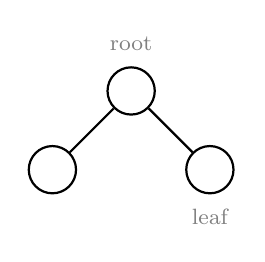
\begin{tikzpicture}

      \tikzset{
        basicnode/.style={
            shape=circle,
            draw=black,
            thick,
            fill=white,
            minimum size=6mm,
            inner sep=0pt
          }
      }

      \node[basicnode] (m1) at (0,0) {};
      \node[basicnode] (m2) at (-1,-1) {};
      \node[basicnode] (m3) at (1,-1) {};

      \node[above of =m1, yshift=-4mm, smallgraytext] {root};
      \node[below of =m3, yshift=4mm, smallgraytext] {leaf};

      \draw[thick] (m1) edge (m2);
      \draw[thick] (m1) edge (m3);
    \end{tikzpicture}
  \end{figure}
\end{frame}

\begin{frame}
  \begin{defboxtop}
    A \highlight{\textbf{tree}} is a collection of nodes, $N$ and branches, $B$, representing connections between nodes.
    \begin{figure}
      \centering
      \begin{tikzpicture}[scale=0.8, transform shape]

        \node[defaultnode] (tB) at (0, 1.5);
        \node[defaultnode] (tA) at (-2, 0);
        \node[defaultnode] (tG) at (0, 0);
        \node[defaultnode] (tC) at (2, 0);
        \node[defaultnode] (tE) at (1, -1.5);
        \node[defaultnode] (tD) at (3, -1.5);

        \draw[defaultnode] (tB) edge (tA);
        \draw[defaultnode] (tB) edge (tG);
        \draw[defaultnode] (tB) edge (tC);
        \draw[defaultnode] (tC) edge (tE);
        \draw[defaultnode] (tC) edge (tD);

      \end{tikzpicture}
    \end{figure}
    \begin{center}
      \graytext{an example tree}
    \end{center}
  \end{defboxtop}
\end{frame}

\begin{frame}
  \begin{defboxside}
    Given a node, $n \in N$, we define:
    \begin{itemize}
      \item $\textsf{pnt}(v) \in N \cup \lbrace \varnothing \rbrace$ as the parent (if it exists)
      \item $\textsf{chl}(v) \subseteq N$ as the set of children
    \end{itemize}
    \begin{figure}
      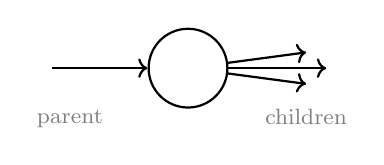
\begin{tikzpicture}
        \node[opacity=0] at (-1.5,0) (l) {$u$};
        \node[defaultnode] at (0,0) (v) {};
        \node[opacity=0] at (1.5, 0) (r) {$w$};


        \node[smallgraytext, below = 2mm of l] {parent};
        \node[smallgraytext, below = 2mm of r] {children};

        \draw[->, defaultnode] (v) -- (r.north);
        \draw[->, defaultnode] (v) -- (r.east);
        \draw[->, defaultnode] (v) -- (r.south);

        \draw[->, defaultnode] (l.west) -- (v);
      \end{tikzpicture}
    \end{figure}
  \end{defboxside}
\end{frame}

\begin{frame}
  \begin{defboxbot}
    An \highlight{\textbf{arborescence}} is a directed tree.
    \\~\\
    \begin{minipage}[t][5cm][t]{0.5\textwidth}
      \begin{center}
        \highlight{\textbf{in-arborescence}}\\
        \footnotesize\color{gray} has a single root node \\ with only incoming branches \\
        \normalsize\color{black}
      \end{center}
      \begin{figure}
        \centering
        \begin{tikzpicture}[scale=0.8, transform shape]

          \node[defaultnode] (tB) at (0, 1.5);
          \node[defaultnode] (tA) at (-2, 0);
          \node[defaultnode] (tG) at (0, 0);
          \node[defaultnode] (tC) at (2, 0);
          \node[defaultnode] (tE) at (1, -1.5);
          \node[defaultnode] (tD) at (3, -1.5);

          \draw[defaultnode, <-] (tB) edge (tA);
          \draw[defaultnode, <-] (tB) edge (tG);
          \draw[defaultnode, <-] (tB) edge (tC);
          \draw[defaultnode, <-] (tC) edge (tE);
          \draw[defaultnode, <-] (tC) edge (tD);

        \end{tikzpicture}
      \end{figure}
    \end{minipage}%
    \begin{minipage}[t][5cm][t]{0.5\textwidth}
      \begin{center}
        \highlight{\textbf{out-arborescence}}\\
        \footnotesize\color{gray} has a single root node \\ with only outgoing branches \\
        \normalsize\color{black}
      \end{center}
      \begin{figure}
        \centering
        \begin{tikzpicture}[scale=0.8, transform shape]

          \node[defaultnode] (tB) at (0, 1.5);
          \node[defaultnode] (tA) at (-2, 0);
          \node[defaultnode] (tG) at (0, 0);
          \node[defaultnode] (tC) at (2, 0);
          \node[defaultnode] (tE) at (1, -1.5);
          \node[defaultnode] (tD) at (3, -1.5);

          \draw[defaultnode, ->] (tB) edge (tA);
          \draw[defaultnode, ->] (tB) edge (tG);
          \draw[defaultnode, ->] (tB) edge (tC);
          \draw[defaultnode, ->] (tC) edge (tE);
          \draw[defaultnode, ->] (tC) edge (tD);

        \end{tikzpicture}
      \end{figure}
    \end{minipage}%
  \end{defboxbot}
\end{frame}

\begin{frame}[fragile]
  A \texttt{Tree} stores \texttt{TreeNode} objects and supports the following operations:\\~\\
  \begin{itemize}

    \item \highlight{\texttt{get\_node}} \\
          \graytext{returns an object (if it exists)}\\[-1mm]
          \begin{lstlisting}[style=mypython]
get_node(key: Key) -> Optional[TreeNode]
\end{lstlisting}

    \item \highlight{\texttt{append\_node}} \\
          \graytext{adds/updates an object as a child of \texttt{pos}}\\[-1mm]
          \begin{lstlisting}[style=mypython]
append_node(key: Key, obj: Object, pos: Key) -> Optional[TreeNode]
\end{lstlisting}

    \item \highlight{\texttt{delete\_node}} \\
          \graytext{removes an object (if it exists) and all sub-objects}\\[-1mm]
          \begin{lstlisting}[style=mypython]
delete_node(key: Key) -> Optional[TreeNode]
\end{lstlisting}

  \end{itemize}
\end{frame}

\begin{frame}{Trees (via Adjacency Lists)}
  \begin{center}
    \Large \highlight{\texttt{Tree}} \\[1mm]
    \normalsize \color{gray} (via Adjacency Lists)
  \end{center}
\end{frame}

\begin{frame}[fragile]
  \begin{thmboxtop}
    \highlight{\texttt{Tree}} \\
    \graytext{(via Adjacency Lists)}
    \begin{lstlisting}[style=mypython]
class TreeNode:
# attributes
    # the key of this node
    key: Key
    
    # the object of this node
    obj: Object

    # the children of this node 
    children: List[TreeNode]

    # the parent of this node
    pnt: Optional[TreeNode]
\end{lstlisting}
  \end{thmboxtop}
\end{frame}

\begin{frame}[fragile]
  \begin{thmboxbot}
    \begin{lstlisting}[style=mypython, firstnumber=last]
class Tree:
# attributes
    # the root
    root: Optional[TreeNode]

    # the number of vertices
    size: Integer

# functions
    ...
\end{lstlisting}
  \end{thmboxbot}
\end{frame}

\begin{frame}[fragile]
  \begin{proofbox}
    \begin{lstlisting}[style=mypython]
def get_node(self: Tree, key: Key) -> Optional[TreeNode]:
    if root is None:
        return None

    stack = Stack()
    stack.push(root)

    while stack.size > 0:
        v = stack.pop()
        if v.key is key:
            return v
        for child in v.children:
            stack.push(child)
    return None
\end{lstlisting}
  \end{proofbox}
\end{frame}

\begin{frame}[fragile]
  \begin{proofbox}
    \begin{lstlisting}[style=mypython]
def append_node(self: Tree, key: Key, obj: Object, pos: Key) -> Optional[TreeNode]:
    pnt = self.get_node(pos)
    if pnt is None:
        return None

    new = TreeNode(key, obj)
    new.pnt = pnt
    pnt.children.append(new)
    return new
\end{lstlisting}
  \end{proofbox}
\end{frame}

\begin{frame}[fragile]
  \begin{proofbox}
    \begin{lstlisting}[style=mypython]
def delete_node(self: Tree, key: Key) -> Optional[TreeNode]:
    vic = self.get_node(key)
    if vic is None:
        return None

    vic.pnt.children.delete(vic.key)
    vic.pnt = None
    return vic
\end{lstlisting}
  \end{proofbox}
\end{frame}

\end{document}
